\documentclass[12pt]{book}
\usepackage[utf8]{inputenc}
\usepackage[T1]{fontenc}
\usepackage{amsmath}
\usepackage{amssymb}
\usepackage{geometry}
\usepackage{tikz}
\usepackage{pgfplots}
\usepackage{xcolor}
\usepackage{mdframed}
\usepackage{enumitem}
\usepackage{booktabs}
\usepackage{array}
\usepackage{fancyhdr}
\usepackage{titlesec}
\pgfplotsset{compat=1.18}
\geometry{margin=1.1in, top=1.2in, bottom=1.2in}

\definecolor{mathblue}{RGB}{30,90,160}
\definecolor{mathgreen}{RGB}{30,140,80}
\definecolor{mathred}{RGB}{180,40,40}
\definecolor{lightgray}{RGB}{240,240,240}

\titleformat{\chapter}[display]
  {\normalfont\large\bfseries}
  {\chaptertitlename\ \thechapter}{12pt}{\LARGE}
\titleformat{\section}
  {\normalfont\large\bfseries}{{\thesection}}{1em}{}
\titleformat{\subsection}
  {\normalfont\normalsize\bfseries}{{\thesubsection}}{1em}{}

\setcounter{chapter}{6}

\pagestyle{fancy}
\fancyhf{}
\fancyhead[LE]{\small\textit{Chapter \thechapter.\
  Continuous Math II: Cost, Revenue, and Profit}}
\fancyhead[RO]{\small\textit{Observing with Mathematical Perspectives}}
\fancyfoot[C]{\small\thepage}
\renewcommand{\headrulewidth}{0.4pt}

\newcounter{exercise}[section]
\renewcommand{\theexercise}{\thesection.\arabic{exercise}}
\newenvironment{exercises}{%
  \begin{mdframed}[backgroundcolor=lightgray, linewidth=0pt,
    innertopmargin=10pt, innerbottommargin=10pt]
  \noindent\textbf{Exercises \thesection}
  \begin{list}{\theexercise.}
    {\usecounter{exercise}
     \setlength{\leftmargin}{2em}
     \setlength{\itemsep}{6pt}}
}{%
  \end{list}
  \end{mdframed}
}

\newcounter{example}[section]
\renewcommand{\theexample}{\thesection.\arabic{example}}
\newenvironment{example}[1][]{%
  \refstepcounter{example}
  \medskip
  \noindent\textbf{Example \theexample.}%
  \ifx&#1&\else\ \textit{(#1)}\fi\quad
}{%
  \medskip
}

\newenvironment{definition}[1]{%
  \begin{mdframed}[linecolor=mathblue, linewidth=1pt,
    innertopmargin=8pt, innerbottommargin=8pt]
  \noindent\textbf{Definition.} \textit{#1.}\quad
}{%
  \end{mdframed}\medskip
}

\begin{document}

%====================================================================
\chapter{Continuous Math II: Cost, Revenue, and Profit}
%====================================================================

This chapter develops three closely related ideas used in
business mathematics: cost, revenue, and profit. Cost describes
how much it takes to produce or operate. Revenue describes the
money brought in from sales. Profit is the difference between
the two.

We begin with linear models in which each additional unit
changes cost or revenue by a constant amount. This leads
naturally to profit functions, break-even analysis, and
marginal analysis. These tools help answer practical questions
such as how many units must be sold to avoid a loss and how
profit changes as production increases.

%--------------------------------------------------------------------
\section{Cost Functions}
%--------------------------------------------------------------------

The total cost of operating a business depends on two
components: costs that are fixed regardless of production
volume, and costs that vary with the number of units produced.

\begin{definition}{Fixed cost}
\textbf{Fixed cost} $F$ is the total cost incurred
regardless of the quantity produced.
Examples include rent, insurance, equipment, and
administrative salaries.
\end{definition}

\begin{definition}{Variable cost}
\textbf{Variable cost} is the cost per unit of production,
denoted $v$.
The total variable cost at quantity $q$ is $v \cdot q$.
\end{definition}

\begin{definition}{Total cost function}
The \textbf{total cost function} is:
\[
C(q) = F + v \cdot q,
\]
where $F$ is fixed cost, $v$ is variable cost per unit,
and $q$ is quantity produced.
\end{definition}

\noindent
The graph of $C(q)$ is a straight line with slope $v$
and vertical intercept $F$. This reflects the fact that each
additional unit adds the same amount, $v$, to the total cost.

\begin{example}
A candle maker pays \$180 per month in fixed costs and
spends \$4 per candle in materials.
\[
C(q) = 180 + 4q.
\]

\begin{center}
\renewcommand{\arraystretch}{1.5}
\begin{tabular}{cc}
\toprule
\textbf{Candles} $q$ & \textbf{Total cost} $C(q)$ \\
\midrule
0   & \$180 \\
20  & \$260 \\
40  & \$340 \\
60  & \$420 \\
80  & \$500 \\
100 & \$580 \\
\bottomrule
\end{tabular}
\end{center}

Each row adds \$80 to the cost, corresponding to
20 additional candles at \$4 each.
\end{example}

\begin{example}[Identifying cost components]
A food truck has the following weekly expenses:
truck payment \$300, insurance \$50, ingredients \$3.50
per meal, packaging \$0.50 per meal.

Fixed cost: $F = 300 + 50 = \$350$.\\
Variable cost: $v = 3.50 + 0.50 = \$4.00$ per meal.\\
Total cost function: $C(q) = 350 + 4q$.

At $q = 200$ meals:
\[
C(200) = 350 + 4(200) = 350 + 800 = \$1{,}150.
\]
\end{example}

\begin{exercises}
  \item Write the cost function $C(q)$ for each situation
    and compute the cost at the given quantity.
    \begin{enumerate}[label=(\alph*), itemsep=5pt]
      \item Fixed cost \$500, variable cost \$8 per unit,
        $q = 75$ units.
      \item Fixed cost \$1{,}200, variable cost \$15 per
        unit, $q = 40$ units.
      \item Monthly rent \$600, utilities \$100, ingredients
        \$2.50 per serving, $q = 300$ servings.
    \end{enumerate}

  \item A bakery has fixed costs of \$250 per week and
    a variable cost of \$1.50 per loaf.
    \begin{enumerate}[label=(\alph*), itemsep=4pt]
      \item Write the cost function.
      \item Fill in the cost table for
        $q = 0, 50, 100, 150, 200$.
      \item By how much does the cost increase for each
        additional 50 loaves?
        What does this amount represent?
    \end{enumerate}

  \item A company's total cost at $q = 100$ units is
    \$1{,}800 and at $q = 200$ units is \$2{,}600.
    Assume the cost function is linear.
    \begin{enumerate}[label=(\alph*), itemsep=4pt]
      \item Find the variable cost per unit.
      \item Find the fixed cost.
      \item Write the cost function $C(q)$.
    \end{enumerate}

  \item A cost function is $C(q) = 400 + 6q$.
    \begin{enumerate}[label=(\alph*), itemsep=4pt]
      \item Identify the fixed cost and variable cost per unit.
      \item Compute $C(0)$ and explain what it represents.
      \item At what quantity does the total cost first
        exceed \$1{,}000?
    \end{enumerate}
\end{exercises}

%--------------------------------------------------------------------
\section{Revenue Functions}
%--------------------------------------------------------------------

\begin{definition}{Revenue function}
The \textbf{revenue function} gives the total income from
selling $q$ units at price $p$ per unit:
\[
R(q) = p \cdot q.
\]
\end{definition}

\noindent
Revenue is also an additive recursion.
Each additional unit sold adds exactly $p$ to revenue,
starting from $R(0) = 0$.
The graph of $R(q)$ is a straight line through the origin
with slope $p$.

\begin{example}
The candle maker from Example 7.1.1 sells each candle for
\$10.
\[
R(q) = 10q.
\]

\begin{center}
\renewcommand{\arraystretch}{1.5}
\begin{tabular}{cc}
\toprule
\textbf{Candles} $q$ & \textbf{Revenue} $R(q)$ \\
\midrule
0   & \$0    \\
20  & \$200  \\
40  & \$400  \\
60  & \$600  \\
80  & \$800  \\
100 & \$1{,}000 \\
\bottomrule
\end{tabular}
\end{center}

Each row adds \$200 to revenue, corresponding to 20
additional candles at \$10 each.
\end{example}

\begin{example}[Finding the price from data]
A lemonade stand takes in \$0 when it sells nothing and
\$120 when it sells 40 cups.
What is the price per cup, and what is the revenue function?
\[
p = \frac{R(q)}{q} = \frac{120}{40} = \$3.00 \text{ per cup.}
\]
\[
R(q) = 3q.
\]
\end{example}

\begin{exercises}
  \item Write the revenue function $R(q)$ for each
    situation and compute revenue at the given quantity.
    \begin{enumerate}[label=(\alph*), itemsep=4pt]
      \item Price \$25 per unit, $q = 60$ units.
      \item Price \$4.50 per item, $q = 200$ items.
      \item Price \$85 per service, $q = 12$ services.
    \end{enumerate}

  \item A food truck earns \$560 selling 80 meals.
    \begin{enumerate}[label=(\alph*), itemsep=4pt]
      \item Find the price per meal.
      \item Write the revenue function.
      \item At what quantity does revenue reach \$1{,}400?
    \end{enumerate}

  \item Two products are sold at different prices.
    Product A sells for \$12 per unit.
    Product B sells for \$20 per unit.
    In one week, 30 units of A and 15 units of B are sold.
    \begin{enumerate}[label=(\alph*), itemsep=4pt]
      \item Compute total revenue from each product.
      \item Compute total revenue from both products combined.
    \end{enumerate}

  \item A revenue function is $R(q) = 18q$.
    A cost function is $C(q) = 240 + 10q$.
    At $q = 40$:
    \begin{enumerate}[label=(\alph*), itemsep=4pt]
      \item Compute $R(40)$ and $C(40)$.
      \item Is revenue greater or less than cost at
        this quantity?
    \end{enumerate}
\end{exercises}

%--------------------------------------------------------------------
\section{Profit and Break-Even}
%--------------------------------------------------------------------

\begin{definition}{Profit function}
The \textbf{profit function} is revenue minus cost:
\[
P(q) = R(q) - C(q) = pq - (F + vq) = (p - v)q - F.
\]
When $P(q) > 0$, the business is profitable. When $P(q) < 0$,
the business is operating at a loss. When $P(q) = 0$, the business
breaks even.
\end{definition}

\noindent
\begin{definition}{Break-even point}
The \textbf{break-even point} is the quantity $q^*$ at which
profit equals zero: $R(q^*) = C(q^*)$. Assume $p > v$, so each
unit contributes a positive amount toward covering fixed costs.
Under this condition,
\[
pq^* = F + vq^* \;\Rightarrow\;
(p - v)q^* = F \;\Rightarrow\;
q^* = \frac{F}{p - v}.
\]
If $F > 0$ and $p \le v$, there is no nonnegative break-even
quantity: each unit contributes no positive amount toward covering
the fixed cost.
\end{definition}

\begin{example}
The candle maker: $F = 180$, $v = 4$, $p = 10$.
\[
P(q) = (10 - 4)q - 180 = 6q - 180.
\]

\begin{center}
\renewcommand{\arraystretch}{1.5}
\begin{tabular}{cccc}
\toprule
$q$ & $C(q)$ & $R(q)$ & $P(q)$ \\
\midrule
0   & \$180 & \$0   & $-\$180$ \\
20  & \$260 & \$200 & $-\$60$  \\
30  & \$300 & \$300 & \$0      \\
40  & \$340 & \$400 & \$60     \\
60  & \$420 & \$600 & \$180    \\
\bottomrule
\end{tabular}
\end{center}

Break-even: $q^* = 180 / 6 = 30$ candles.
At 30 candles the maker covers all costs exactly.
At fewer than 30, a loss results.
At more than 30, a profit results.
\end{example}

\begin{example}
A food truck: $F = 350$, $v = 4$, $p = 8$.
\[
P(q) = (8 - 4)q - 350 = 4q - 350.
\]
\[
q^* = \frac{350}{8 - 4} = \frac{350}{4} = 87.5.
\]
Since the truck cannot sell half a meal, the break-even
quantity rounds up to $q^* = 88$ meals.
At 88 meals:
\[
P(88) = 4(88) - 350 = 352 - 350 = \$2 \text{ profit.}
\]
\end{example}

\begin{center}
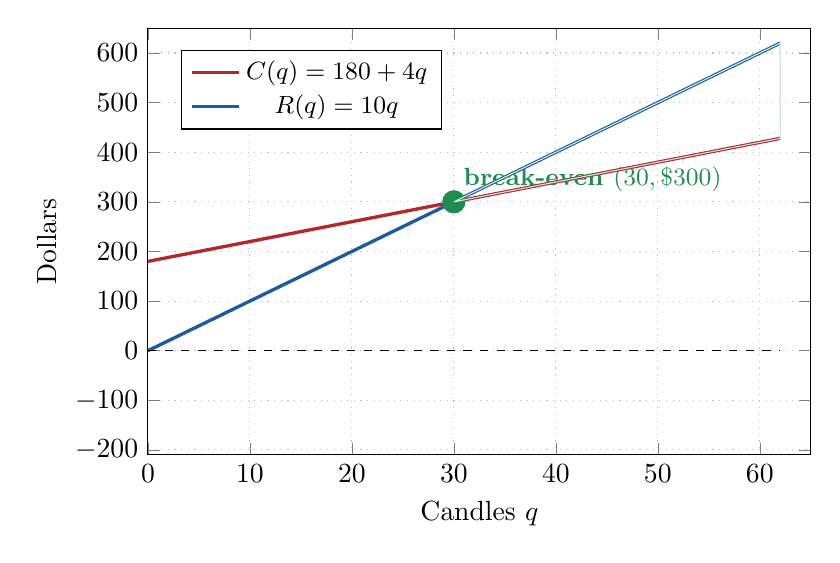
\begin{tikzpicture}
\begin{axis}[
  width=10cm, height=7cm,
  xlabel={Candles $q$},
  ylabel={Dollars},
  xtick={0,10,20,30,40,50,60},
  ytick={-200,-100,0,100,200,300,400,500,600},
  ymin=-210, ymax=650,
  xmin=0, xmax=65,
  grid=major, grid style=dotted,
  legend style={at={(0.05,0.95)}, anchor=north west, font=\small},
]
% Cost line C(q) = 180 + 4q
\addplot[mathred, very thick, domain=0:62]
  {180 + 4*x};
\addlegendentry{$C(q) = 180 + 4q$}

% Revenue line R(q) = 10q
\addplot[mathblue, very thick, domain=0:62]
  {10*x};
\addlegendentry{$R(q) = 10q$}

% Break-even point
\filldraw[mathgreen] (axis cs:30,300) circle (4pt);
\node[above right, mathgreen, font=\small\bfseries]
  at (axis cs:30,300) {break-even $(30, \$300)$};

% Profit shading (approximate)
\addplot[mathgreen!20, fill opacity=0.35]
  coordinates {(30,300)(62,620)(62,428)(30,300)};

% Zero profit line
\draw[black, dashed, thin] (axis cs:0,0)--(axis cs:62,0);
\end{axis}
\end{tikzpicture}
\end{center}

\begin{exercises}
  \item For each situation, write the profit function,
    find the break-even quantity, and compute the profit
    or loss at the given quantity.
    \begin{enumerate}[label=(\alph*), itemsep=5pt]
      \item $F = \$300$, $v = \$5$, $p = \$11$,
        find $P(80)$.
      \item $F = \$600$, $v = \$8$, $p = \$14$,
        find $P(120)$.
      \item $F = \$1{,}000$, $v = \$12$, $p = \$20$,
        find $P(100)$.
    \end{enumerate}

  \item A student sells handmade greeting cards at a craft
    fair.
    The table fee is \$48 and each card costs \$1.50 to make.
    Cards sell for \$6 each.
    \begin{enumerate}[label=(\alph*), itemsep=4pt]
      \item Write $C(q)$, $R(q)$, and $P(q)$.
      \item Find the break-even quantity.
      \item Complete the profit table for
        $q = 0, 8, 10, 12, 16, 20$.
      \item How much profit is earned at $q = 20$?
    \end{enumerate}

  \item A company's profit function is $P(q) = 7q - 420$.
    \begin{enumerate}[label=(\alph*), itemsep=4pt]
      \item Find the break-even quantity.
      \item Identify the fixed cost and the profit per unit
        beyond break-even.
      \item At what quantity does profit reach \$280?
    \end{enumerate}

  \item A business has fixed costs of \$500 and earns
    \$5 profit on each unit sold beyond break-even.
    At $q = 120$ units the business earns a profit of
    \$100.
    \begin{enumerate}[label=(\alph*), itemsep=4pt]
      \item Find the break-even quantity.
      \item Find the price per unit and variable cost per
        unit, given that $p - v = \$5$.
        \textit{Hint: use the formula for $q^*$.}
    \end{enumerate}
\end{exercises}

%--------------------------------------------------------------------
\section{Marginal Analysis}
%--------------------------------------------------------------------

\begin{definition}{Marginal cost}
The \textbf{marginal cost} is the cost of producing one
additional unit.
For the linear cost function $C(q) = F + vq$, the marginal
cost equals the variable cost per unit $v$.
\end{definition}

\begin{definition}{Marginal revenue}
The \textbf{marginal revenue} is the revenue from selling
one additional unit.
For the linear revenue function $R(q) = pq$, the marginal
revenue equals the price $p$.
\end{definition}

\begin{definition}{Marginal profit}
The \textbf{marginal profit} is the profit gained from
selling one additional unit.
\[
\text{Marginal profit} = p - v.
\]
\end{definition}

\noindent
The marginal profit is the step size of the profit recursion.
Each additional unit sold beyond break-even adds exactly
$p - v$ to profit.
This is the additive recursion from Chapter 1, now describing
profit growth.

\begin{example}
For the candle maker: $p = 10$, $v = 4$.
\[
\text{Marginal profit} = 10 - 4 = \$6 \text{ per candle.}
\]
Every candle sold beyond the break-even point of 30
adds \$6 to profit.

At $q = 50$: the business is $50 - 30 = 20$ candles beyond
break-even.
\[
P(50) = 6 \times 20 = \$120.
\]
Verification: $P(50) = 6(50) - 180 = 300 - 180 = \$120$.
\checkmark
\end{example}

\begin{example}[Marginal analysis at the boundary]
A print shop has $C(q) = 500 + 2q$ and $R(q) = 6q$.
\[
\text{Marginal cost} = \$2, \quad
\text{Marginal revenue} = \$6, \quad
\text{Marginal profit} = \$4.
\]
Break-even: $q^* = 500 / 4 = 125$ prints.

At $q = 124$: one unit below break-even.
\[
P(124) = 4(124) - 500 = 496 - 500 = -\$4.
\]

At $q = 125$: break-even.
\[
P(125) = 4(125) - 500 = 0.
\]

At $q = 126$: one unit above break-even.
\[
P(126) = 4(126) - 500 = \$4.
\]

Each unit past break-even adds exactly \$4 of profit,
confirming that \$4 is the step size of the profit recursion.
\end{example}

\begin{example}[Comparing two pricing strategies]
A market vendor considers two pricing options for handmade
soap.

\begin{center}
\renewcommand{\arraystretch}{1.5}
\begin{tabular}{lcc}
\toprule
& \textbf{Strategy A} & \textbf{Strategy B} \\
\midrule
Price per bar       & \$8  & \$12 \\
Variable cost       & \$3  & \$3  \\
Fixed cost          & \$200 & \$200 \\
Marginal profit     & \$5  & \$9  \\
Break-even quantity & 40   & 22.2 $\approx$ 23 \\
\bottomrule
\end{tabular}
\end{center}

Strategy B reaches break-even faster.
At $q = 40$:
\[
P_A(40) = 5(40) - 200 = \$0, \quad
P_B(40) = 9(40) - 200 = \$160.
\]

Strategy B produces substantially more profit at the same
volume.
However, the higher price may reduce the number of buyers.
Marginal analysis quantifies the profit per unit sold;
it does not predict how many units will sell.
\end{example}

\begin{exercises}
  \item Find the marginal cost, marginal revenue, and
    marginal profit for each situation.
    \begin{enumerate}[label=(\alph*), itemsep=4pt]
      \item $C(q) = 300 + 7q$, $R(q) = 15q$
      \item $C(q) = 800 + 20q$, $R(q) = 35q$
      \item $F = \$450$, $v = \$9$, $p = \$14$
    \end{enumerate}

  \item A craft fair vendor has marginal profit of \$6
    per item and fixed costs of \$240.
    \begin{enumerate}[label=(\alph*), itemsep=4pt]
      \item Find the break-even quantity.
      \item How much profit is earned at 10 items beyond
        break-even?
      \item At what quantity does profit reach \$120?
    \end{enumerate}

  \item Two businesses have the same fixed cost of \$600.
    Business A has marginal profit \$10 per unit.
    Business B has marginal profit \$15 per unit.
    \begin{enumerate}[label=(\alph*), itemsep=4pt]
      \item Find the break-even quantity for each.
      \item At $q = 80$ units, compute the profit for each.
      \item Which business benefits more from selling
        10 additional units beyond $q = 80$?
        Compute the difference.
    \end{enumerate}

  \item Explain in two complete sentences the connection
    between marginal profit and the additive recursion
    introduced in Chapter 1.
    Use a specific numerical example to support your
    explanation.
\end{exercises}

%--------------------------------------------------------------------
\section{Graphical Analysis}
%--------------------------------------------------------------------

The cost and revenue functions are both straight lines.
Their graph reveals the complete structure of the profit
situation at a glance.

\begin{enumerate}[itemsep=5pt]
  \item The \textbf{vertical intercept} of the cost line
    is the fixed cost $F$.
    The cost line never passes through the origin unless
    $F = 0$.

  \item The \textbf{revenue line} always passes through
    the origin: at $q = 0$, revenue is zero.

  \item The \textbf{break-even point} is the intersection
    of the two lines.

  \item For quantities \textbf{to the left} of the
    break-even point, the cost line is above the revenue
    line: the business is at a loss.

  \item For quantities \textbf{to the right} of the
    break-even point, the revenue line is above the cost
    line: the business is profitable.

  \item The \textbf{slope} of the revenue line is the
    price $p$.
    The \textbf{slope} of the cost line is the variable
    cost $v$.
    The profit per additional unit is the difference in
    slopes: $p - v$.
\end{enumerate}

\begin{example}
Graph the cost and revenue functions for a tutoring service:
$F = \$200$, $v = \$5$ per hour, $p = \$25$ per hour.
\[
C(q) = 200 + 5q, \quad R(q) = 25q.
\]
Break-even: $q^* = 200 / 20 = 10$ hours.

\begin{center}
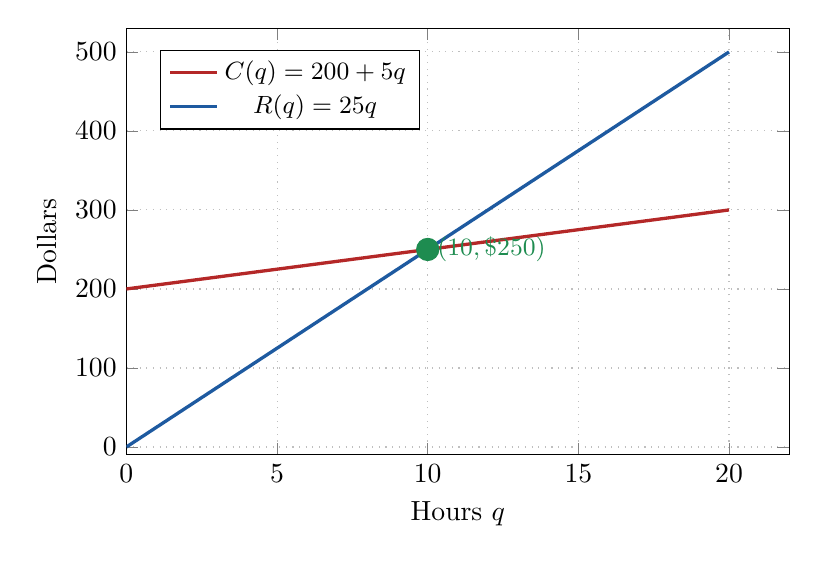
\begin{tikzpicture}
\begin{axis}[
  width=10cm, height=7cm,
  xlabel={Hours $q$},
  ylabel={Dollars},
  xtick={0,5,10,15,20},
  ytick={0,100,200,300,400,500},
  ymin=-10, ymax=530,
  xmin=0, xmax=22,
  grid=major, grid style=dotted,
  legend style={at={(0.05,0.95)}, anchor=north west, font=\small},
]
\addplot[mathred, very thick, domain=0:20]
  {200 + 5*x};
\addlegendentry{$C(q) = 200 + 5q$}
\addplot[mathblue, very thick, domain=0:20]
  {25*x};
\addlegendentry{$R(q) = 25q$}
\filldraw[mathgreen] (axis cs:10,250) circle (4pt);
\node[right, mathgreen, font=\small\bfseries]
  at (axis cs:10,250) {$(10, \$250)$};
\end{axis}
\end{tikzpicture}
\end{center}

The revenue line rises more steeply than the cost line
because $p > v$.
Beyond the intersection at $q = 10$ hours, revenue exceeds
cost and the tutor earns a profit.
\end{example}

\begin{example}[Reading the graph]
A graph shows two lines.
The cost line has vertical intercept \$400 and passes
through the point $(50, \$650)$.
The revenue line passes through the origin and the point
$(50, \$750)$.

From the cost line:
\[
v = \frac{650 - 400}{50 - 0} = \frac{250}{50} = \$5 \text{ per unit.}
\]
\[
C(q) = 400 + 5q.
\]

From the revenue line:
\[
p = \frac{750}{50} = \$15 \text{ per unit.}
\]
\[
R(q) = 15q.
\]

Break-even:
\[
q^* = \frac{400}{15 - 5} = \frac{400}{10} = 40 \text{ units.}
\]
\end{example}

\begin{exercises}
  \item For each pair of functions, identify the fixed cost,
    variable cost, price, and break-even quantity by
    reading the equations.
    Then sketch the graph, labeling both lines and the
    break-even point.
    \begin{enumerate}[label=(\alph*), itemsep=6pt]
      \item $C(q) = 150 + 3q$, $\quad R(q) = 9q$
      \item $C(q) = 400 + 10q$, $\quad R(q) = 18q$
      \item $C(q) = 600 + 12q$, $\quad R(q) = 20q$
    \end{enumerate}

  \item A graph of cost and revenue functions shows the
    following:
    \begin{itemize}[itemsep=2pt]
      \item The cost line crosses the vertical axis at
        \$300.
      \item The cost line passes through $(60, \$660)$.
      \item The revenue line passes through $(60, \$900)$.
    \end{itemize}
    \begin{enumerate}[label=(\alph*), itemsep=4pt]
      \item Write $C(q)$ and $R(q)$.
      \item Find the break-even quantity.
      \item Find the profit at $q = 80$.
    \end{enumerate}

  \item Two businesses sell the same product at the same
    price of \$20 per unit.
    Business A has fixed costs of \$800 and variable
    costs of \$8 per unit.
    Business B has fixed costs of \$400 and variable
    costs of \$12 per unit.
    \begin{enumerate}[label=(\alph*), itemsep=4pt]
      \item Write the profit function for each business.
      \item Find the break-even quantity for each.
      \item At $q = 60$, which business is more profitable?
        By how much?
      \item Sketch both profit functions on the same axes.
        At what quantity do they produce equal profit?
    \end{enumerate}
\end{exercises}

%--------------------------------------------------------------------
\section{The Observer and the Business}
%--------------------------------------------------------------------

A cost, revenue, and profit analysis describes the same
operation from the perspective of the numbers alone.
Different observers read different quantities from that
analysis because they are asking different questions.

\begin{center}
\renewcommand{\arraystretch}{1.5}
\begin{tabular}{ll}
\toprule
\textbf{Observer} & \textbf{Primary question} \\
\midrule
Business owner &
  How many units must I sell to cover costs? \\
Investor &
  At what volume does this become profitable? \\
Operations manager &
  What does each additional unit cost to produce? \\
Pricing strategist &
  How does a price change affect break-even? \\
Customer &
  What is the price per unit? \\
\bottomrule
\end{tabular}
\end{center}

\noindent
Each question is answered by a different quantity extracted
from the same three functions.
The break-even quantity answers the owner's question.
The marginal profit answers the investor's question about
per-unit profitability.
The variable cost answers the operations manager's question.
The price answers the customer's question.

\medskip
\noindent
A change in any one parameter propagates through all three
functions.
Raising the price $p$ increases marginal profit, lowers
the break-even quantity, and increases profit at every
$q > q^*$.
Raising the fixed cost $F$ raises the break-even quantity
without changing marginal profit.
An observer focused on only one output may miss consequences
visible to another.

\begin{example}
A food cart currently operates with:
$F = \$350$, $v = \$4$, $p = \$9$.
\[
q^* = \frac{350}{9 - 4} = 70 \text{ meals.}
\]
At $q = 100$: $P(100) = 5(100) - 350 = \$150$.

The owner considers two changes.

\textbf{Option A}: raise the price to \$11.
\[
q^*_A = \frac{350}{11 - 4} = 50 \text{ meals.} \quad
P_A(100) = 7(100) - 350 = \$350.
\]

\textbf{Option B}: reduce fixed cost to \$250 by moving
to a smaller location.
\[
q^*_B = \frac{250}{9 - 4} = 50 \text{ meals.} \quad
P_B(100) = 5(100) - 250 = \$250.
\]

Both options lower the break-even point to 50 meals.
At $q = 100$, Option A produces more profit (\$350 vs.
\$250) because the marginal profit is higher.
The investor asking about per-unit profitability would
prefer Option A.
The operations manager asking about overhead would prefer
Option B.
The customer asking about price would prefer neither.
\end{example}

\begin{exercises}
  \item A business has $C(q) = 420 + 6q$ and $R(q) = 14q$.
    \begin{enumerate}[label=(\alph*), itemsep=4pt]
      \item Find the break-even quantity and profit at
        $q = 80$.
      \item The owner raises the price to \$18.
        Find the new break-even quantity and profit at
        $q = 80$.
      \item The owner instead reduces fixed costs by \$120.
        Find the new break-even quantity and profit at
        $q = 80$ (using the original price of \$14).
      \item Write one sentence comparing the two options
        from the perspective of the break-even quantity.
      \item Write one sentence comparing the two options
        from the perspective of profit at $q = 80$.
    \end{enumerate}

  \item A nonprofit sells event tickets to cover operating
    costs.
    Fixed costs are \$1{,}200.
    Variable costs are \$8 per attendee.
    Ticket price is \$20 per attendee.
    \begin{enumerate}[label=(\alph*), itemsep=4pt]
      \item Find the break-even attendance.
      \item The nonprofit wants to reduce the ticket price
        to \$15 to attract more attendees.
        Find the new break-even attendance.
      \item Write one sentence explaining what the
        nonprofit must consider when choosing between
        the two ticket prices.
    \end{enumerate}
\end{exercises}

%--------------------------------------------------------------------
\section*{Chapter 7 Review}
%--------------------------------------------------------------------

\addcontentsline{toc}{section}{Chapter 7 Review}

\begin{enumerate}[label=\arabic*., leftmargin=2em, itemsep=8pt]

  \item A small printing company has monthly fixed costs
    of \$800 and a variable cost of \$3 per pamphlet.
    Pamphlets sell for \$8 each.
    \begin{enumerate}[label=(\alph*), itemsep=4pt]
      \item Write $C(q)$, $R(q)$, and $P(q)$.
      \item Find the break-even quantity.
      \item Complete the table for $q = 0, 80, 160, 200,
        240$.
      \item Compute the profit at $q = 240$.
    \end{enumerate}

  \item A mobile car wash has fixed costs of \$600 and
    charges \$25 per car.
    Supplies cost \$7 per car.
    \begin{enumerate}[label=(\alph*), itemsep=4pt]
      \item Write all three functions and find the
        break-even quantity.
      \item Find the marginal profit and explain what it
        means in context.
      \item How many cars must be washed to earn a
        \$360 profit?
    \end{enumerate}

  \item A cost function is $C(q) = 900 + 12q$ and a
    revenue function is $R(q) = 21q$.
    \begin{enumerate}[label=(\alph*), itemsep=4pt]
      \item Find the break-even quantity.
      \item Sketch the graph, labeling the vertical
        intercept, the break-even point, and the slopes
        of both lines.
      \item What is the profit at $q = 150$?
    \end{enumerate}

  \item A freelance designer charges \$80 per hour
    and has fixed monthly costs of \$320.
    The designer's time costs \$20 per hour (opportunity
    cost and materials).
    \begin{enumerate}[label=(\alph*), itemsep=4pt]
      \item Write the profit function.
      \item Find the break-even number of hours.
      \item How many hours must be billed to earn
        \$1{,}000 profit per month?
    \end{enumerate}

  \item A business currently sells a product for \$16
    with variable cost \$7 and fixed cost \$540.
    A competitor enters the market, forcing the price
    down to \$13.
    \begin{enumerate}[label=(\alph*), itemsep=4pt]
      \item Find the original break-even quantity
        and profit at $q = 80$.
      \item Find the new break-even quantity and
        profit at $q = 80$ with the lower price.
      \item By how much does the break-even quantity
        increase as a result of the price decrease?
    \end{enumerate}

  \item Two bakeries both sell bread for \$7 per loaf.
    Bakery A: $F = \$400$, $v = \$2$.
    Bakery B: $F = \$200$, $v = \$4$.
    \begin{enumerate}[label=(\alph*), itemsep=4pt]
      \item Write the profit function for each.
      \item Find the break-even quantity for each.
      \item At what quantity do the two bakeries earn
        equal profit?
        (Set $P_A(q) = P_B(q)$ and solve.)
      \item Which bakery is more profitable at high volume?
        Explain using marginal profit.
    \end{enumerate}

  \item Explain in three complete sentences how the
    cost, revenue, and profit functions in this chapter
    are each examples of the additive recursion from
    Chapter 1.
    Identify the starting value and step size for each.

\end{enumerate}

\end{document}
